\section{Experiments and what they establish}
\label{sec:experiments}

\subsection{Pinned corpus comparison}
The baseline is the supplied-cut entry point at \basecommit, loaded from
that exact Git object.  Its dependencies are held at the same revision.
The corpus is the 106-case \code{marked_parallelity_research/corpus.json}.
Its SHA-256 digest and the baseline entry-point digest are recorded in
\code{results/native/native_audit.json}.  Every result records a case label,
statuses, timing scope, census when present, and certificate information.

\begin{table}[htbp]
\centering
\caption{Native supplied-cut census coverage at the pinned revision.}
\label{tab:coverage}
\begin{tabular}{lrr}
\toprule
Outcome & Baseline & With dual normalization\\
\midrule
Complete censuses & 85 & 92\\
Inconclusive cuts & 21 & 14\\
Earlier complete censuses preserved & -- & 85\\
Successful independent certificate replays & -- & 92\\
New censuses agreeing with Regina & -- & 7\\
\bottomrule
\end{tabular}
\end{table}

The coverage rises from $80.19\%$ to $86.79\%$.  Seven of the 21
previously inconclusive cuts become complete, reducing that count by one
third.  This is a measured coverage improvement on supplied cuts.  It is
not a measured speed-up of the end-to-end knot recognizer, and a previous
inconclusive return is not a valid fast baseline for a newly completed
query.  The README's older success count is stale; the comparison uses
the measured 85 rather than that prose count.

\begin{table}[htbp]
\centering\small
\caption{All seven newly certified cuts.  The notation $g^m$ means
$m$ components of genus $g$, not exponentiation.}
\label{tab:new-cuts}
\begin{tabular}{p{0.69\textwidth}l}
\toprule
Corpus label & Genus census\\
\midrule
\code{pilot/interior_1_2/0} & $1^2$\\
\code{pilot/interior_2_3/0} & $1^2$\\
\code{pilot/interior_3_5/0} & $1^1$\\
\code{pilot/finite_trefoil_interior/0} & $2^1$\\
\code{interior_1_2/mixed} & $0^2$\\
\code{interior_3_5/mixed} & $0^2$\\
\code{finite_figureEight_interior/mixed} & $0^1,2^2$\\
\bottomrule
\end{tabular}
\end{table}

The package retains the seven full source/certificate packets.  The audit's
sorted-key JSON encodings of the seven composite certificates alone range
from 11,631 to 1,069,420 bytes.  The
last, larger certificate mainly reflects existing source and boundary
proofs, not a large dual tree.  All seven affected native trees have one
edge in this corpus.  Separate subdivision fixtures exercise many
three-handles, so the tests of the graph stage are not confined to
one-edge cancellation.

\subsection{Which matrices need more than the polynomial theorem?}
The matrix audit first fixes the native lower zero-/one-handle spanning
forest and reads the original source two-handle cycles.  Of the 106
matrices, 12 have maximum column support zero, seven have maximum support
one, 62 have maximum support two, and 25 have maximum support three.
Thus 81 of 106 satisfy the two-row condition before adding interface
relations.  The audit also checks that the total raw occurrence count
of every original source column is at most three.

A separate source-parity audit uses uncapped attaching-cycle counts and an
independently oriented cap oracle.  It checks 3,239 original one-handle
columns and 783 source two-handle rows across the 106 sources, including
columns later removed by the lower forest.  It finds no violation of
either Proposition~\ref{prop:three} or Proposition~\ref{prop:cycle}.
Of 74 triple-unit columns, seven give a parallel pair plus a loop and
67 give three loops.  The corpus has at most one interior vertex per
source, so it cannot test genuine dual triangles.  Three separately
labelled supplementary stellar sources with two, four, and eight interior
vertices provide respectively three, nine, and 25 triangle columns;
all pass the same independent check.  These supplemental sources are
not counted as additional members of the 106-case coverage corpus.

There are ten cuts with three-handles.  Seven of their bare core matrices
are in the polynomial regime, and the polynomial solver finds and verifies
a successful tree in all seven.  The other three bare core matrices also
have successful trees, found and independently checked by the general
stopping search.  \emph{All ten bare cores are therefore solvable in the
fixed raw model.}  This does not settle the actual cuts, because the
parallelity attachments still contribute relations.

The audit next inserts the same finite annular relations used by the
boundary kernel.  Four of these ten augmented matrices satisfy the
polynomial hypothesis.  General forest search succeeds on exactly the
seven cuts of Table~\ref{tab:new-cuts}; it certifies \code{NO_FOREST} on
the other three.  In each negative case there is a stopping witness
consisting entirely of nondeletable interface rows:
\begin{table}[htbp]
\centering\small
\caption{Obstructions that no change of dual tree can remove in the
fixed augmented matrix.  Row identifiers refer to the saved source problem.}
\label{tab:interfaces}
\begin{tabular}{p{0.62\textwidth}ll}
\toprule
Corpus label & Stopping rows & Eligible rank\\
\midrule
\code{pilot/finite_figureEight_interior/0} & $26,\ldots,32$ & $0$\\
\code{interior_2_3/mixed} & $11,\ldots,14$ & $0$\\
\code{finite_trefoil_interior/mixed} & $16$ & $0$\\
\bottomrule
\end{tabular}
\end{table}
Each displayed set is a single nonempty stopping set with no eligible
dual edge.  It is therefore already an obstruction by
Theorem~\ref{thm:transversal}; no exponential negative search is needed
to check it.  This evidence changes the practical research priority:
trying additional dual trees cannot resolve these three fixed kernels.
The attachment treatment or the permitted lower-handle moves must change.

The fourteen remaining native inconclusive cases divide into eight raw
cancellation stalls, three stalls in the boundary kernel after dual
reduction, and three raw ball-cancellation obstructions.  The exact
reason codes are retained in the JSON audit.  These are pipeline outcomes,
not a classification of the underlying knots.

\subsection{Complete-query timings on a parallel-surface family}
We compare two routes to the same component genus census for multiples
of a one-sided normal surface in a finite solid-torus fixture with an
interior vertex.  The native timed route includes certificate production
and independent replay.  The Regina route includes source conversion,
cutting along the normal surface, constructing connected components, and
exact handlebody recognition of those components.  It materializes the
cut triangulation; the native route retains multiplicities in its
compressed census.  JSON serialization, interpreter startup, and import
time are outside both timed arms.

There are five randomized paired rounds at each size, seed 20261012,
using \code{perf_counter}.  The recorded environment is Python 3.12.14,
Regina 7.4, Linux 6.18.44 on x86-64.  Table~\ref{tab:native-timing}
reports median total times and the median of the five within-pair time
ratios.  The latter need not equal the ratio of the two marginal medians.
Raw rounds and stage timings are included; five rounds are too few for
strong distributional claims.

\begin{table}[htbp]
\centering\small
\caption{Complete supplied-cut queries, milliseconds.  A ratio above one
favors the native certified route.}
\label{tab:native-timing}
\begin{tabular}{rrrrrr}
\toprule
Copies & Components & Cut tetrahedra & Native & Regina & Paired ratio\\
\midrule
1 & 1 & 91 & 4.056 & 0.895 & 0.225\\
4 & 3 & 151 & 26.507 & 1.420 & 0.0528\\
16 & 9 & 391 & 27.514 & 3.014 & 0.107\\
64 & 33 & 1,351 & 28.289 & 8.825 & 0.317\\
256 & 129 & 5,191 & 40.501 & 42.282 & 1.044\\
1,024 & 513 & 20,551 & 35.723 & 169.545 & 4.824\\
\bottomrule
\end{tabular}
\end{table}

Regina is much faster on small inputs, by almost a factor of nineteen at
four copies.  The routes are close at 256 copies, and the native route
is about 4.8 times faster at 1,024 copies.  The nonmonotone native timings
show fixed costs and runtime variation; they are not a fitted asymptotic
law.  The asymptotic statement for the new graph stage follows from
Theorem~\ref{thm:native}, not from extrapolating this table.  The comparison
also does not rule out a different compressed implementation using Regina
components or alternative exact recognition procedures.

\begin{figure}[htbp]
\centering
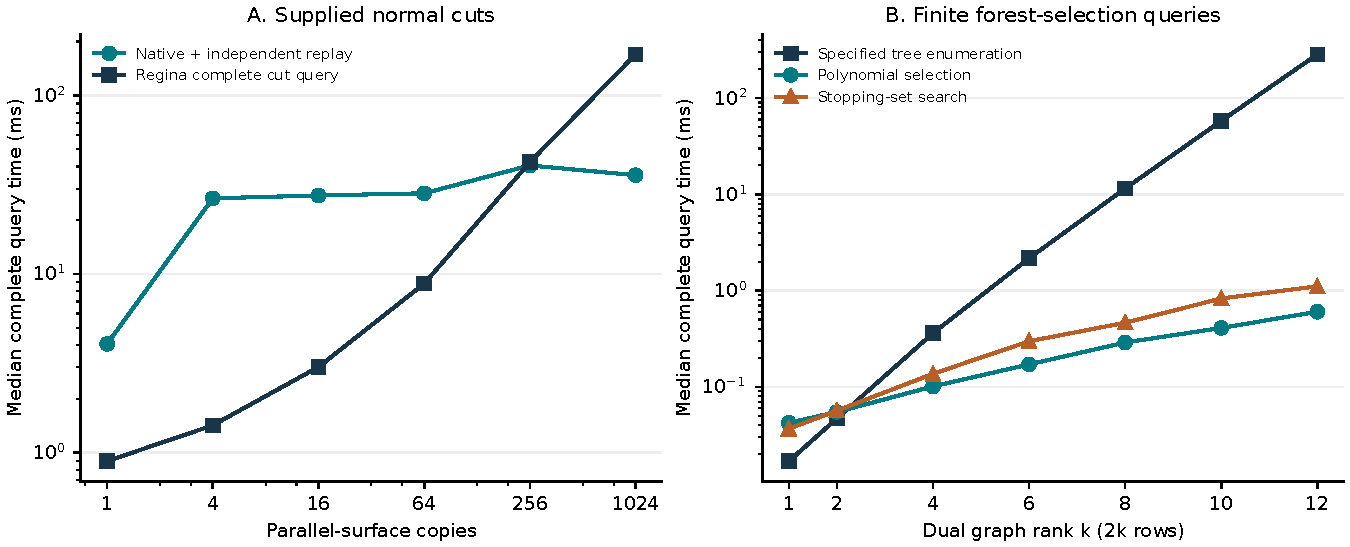
\includegraphics[width=\textwidth]{figures/benchmarks.pdf}
\caption{Recorded complete-query medians.  Left: supplied native cuts,
including independent replay, against the stated Regina route.  Right:
the finite forest-selection family, including the same positive checker
in every arm.  The two panels have different inputs and must not be
combined into a knot-recognition speed-up.}
\label{fig:benchmarks}
\end{figure}

\subsection{Finite decision audit and a controlled enumeration comparison}
The independent finite audit checks 33,995 graph/matrix problems.  Of these,
26,995 are exhaustive enumerations in the stated small families and 7,000
are seeded random cases.  The separate oracle finds 4,554 feasible and
29,441 infeasible instances.  Every general-search certificate replays.
The polynomial solver completes and verifies 23,849 instances; it declines
the other 10,146 because an active column has more than two owners.
These are finite graph/matrix tests, not 33,995 normal-surface examples.

For a controlled comparison, take a chain of $k$ dual links, each replaced
by two parallel edges $a_i,b_i$.  Column $i$ has its sole occurrences on
these two rows, with counts $1$ and $2$, equivalently the capped form of
counts $1$ and $3$.  There are $2^k$ spanning trees.
Every $\{b_i\}$ is a mandatory stopping singleton, so the sole successful
tree is $\{b_1,\ldots,b_k\}$.  The specified include-before-exclude
enumerator, with $a_i$ before $b_i$, reaches this tree last and tests exactly
$2^k$ complete trees.  Stopping search makes $k$ forced choices; the
polynomial solver finds $k$ source-component representatives.  This proves
an exponential separation from that explicit enumeration policy, not a
lower bound against all algorithms.

\begin{table}[htbp]
\centering\small
\caption{Finite forest-selection complete queries, median milliseconds
over five paired rounds.  Every positive arm includes independent replay.}
\label{tab:forest-timing}
\begin{tabular}{rrrrr}
\toprule
$k$ & Trees tested by enumeration & Enumeration & Polynomial & Stopping search\\
\midrule
1 & 2 & 0.0169 & 0.0424 & 0.0368\\
2 & 4 & 0.0470 & 0.0549 & 0.0567\\
4 & 16 & 0.3616 & 0.1012 & 0.1367\\
6 & 64 & 2.1693 & 0.1713 & 0.2978\\
8 & 256 & 11.4927 & 0.2890 & 0.4642\\
10 & 1,024 & 57.8562 & 0.4096 & 0.8278\\
12 & 4,096 & 283.8067 & 0.6030 & 1.1089\\
\bottomrule
\end{tabular}
\end{table}

At $k=12$ the polynomial query is about 470.6 times faster than the
specified enumerator.  At $k=1$ it is about 2.5 times slower.  An identical
enumerator control gives an A/A median-time ratio of 0.987 at $k=12$.
The larger polynomial-only run reaches $k=128$ in 224.3 milliseconds,
including replay.  The hypothetical $2^{128}$ enumeration count there
is a formula, not a measured enumeration run.  Structural visit counters
are included for reproducibility; their totals are not CPU instruction
counts and should not be equated across implementations.

\subsection{Stress tests and remaining measurement limits}
The native focused suite constructs successive interior subdivisions,
exercising up to sixteen interior vertices, as well as normal multiplicity
$2^{4096}$.  It checks a compressed exact census and replay without
enumerating that many normal pieces.  The large-integer case tests the
encoded interface; it does not by itself prove a uniform time bound for
all large-coordinate inputs.  The general finite suite separately tests
huge sparse namespaces and resource exhaustion.

The full repository regression suite passes 1,688 tests in the recorded
run (374.807 seconds).  The standalone finite suite adds 18 focused test
methods; the ten new native methods are included in the 1,688.  The first
sparse checkout lacked historical report fixtures
needed by older tests; those dependencies were restored before the final
regression run.  This setup failure is recorded separately from the final
run and was not counted as a source-code defect or hidden by changing
the tests.  No peak-memory comparison, realistic knot-distribution benchmark,
or end-to-end diagram-recognition timing is claimed in this work.
